%% -*- coding: utf-8-unix -*-

\chapter{NetTesterの技術仕様}
\label{chap:nettester-design}

本プロジェクトでNetTesterに実装した「パッチ」動作とフロー制御方式につい
て解説する。テスト用ノードの操作についてはTrema/Phutを利用して実装されて
いる。Phutの使いかたやNetTesterでの応用については\ref{sec:phut_basics}を
参照のこと。

 \section{NetTesterのモデル}
 \label{sec:nettester-model}

 \subsection{基本的な構成要素}
 \label{sec:nettester-model}

%  NetTester の構成(モデル)
% つかっている技術:
% \begin{itemize}
%  \item network namespaceとその操作, trema/phut
%        \begin{itemize}
%         \item Phut Memo – NetTester \url{https://3.basecamp.com/3088280/buckets/867009/documents/238439817}
%        \end{itemize}
%  \item patch panel 実装, ActiveFlow
%        \begin{itemize}
%         \item パッチの概要 → パッチ – NetTester \url{https://3.basecamp.com/3088280/buckets/867009/documents/213266851}
%         \item "patch panel" model – NetTester \url{https://3.basecamp.com/3088280/buckets/867009/documents/208275139}
%        \end{itemize}
% \end{itemize}
% phut, activeflowなどの実装寄りのはなしは付録とかにするか。

本プロジェクトでは、\ref{sec:basic-tester-idea}節で解説したネットワーク
テストシステムのアイディアを、NetTester~\cite{nettester}というツールとし
て実装した。NetTester は\figref{fig:model-nettester}の示すコンポーネント
で構成される。

\begin{figure}[h]
 \centering
 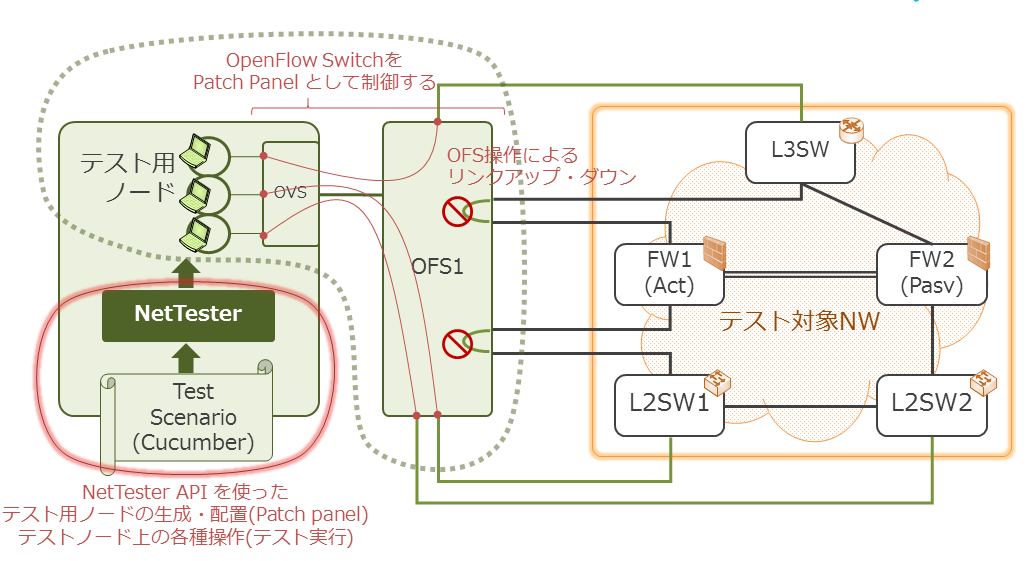
\includegraphics[scale=0.6]{img/model-nettester.png}
 \caption{NetTesterのモデル}
 \label{fig:model-nettester}
\end{figure}

% TODO: PSW, SSWなどの用語にもとづいて図の中身を修正すること

\begin{description}
 \item[物理スイッチ(OFS)] パッチパネルとして動作させるOpenFlowスイッチ
            \footnote{本書あるいはNetTester関連ドキュメント中では ''物理
            OpenFlowスイッチ'',``Physical (OpenFlow) Switch'',''PSW''な
            どで表記される。実装上はPica8スイッチを使用していることから、
            単に''Pica8''とすることがある。}。テスト対象ネットワークのト
            ポロジ操作やテスト用ノードの配置などをおこなう、物理ポートを
            複数もつスイッチである。
 \item[ソフトウェアスイッチ(OVS)] パッチパネルとして動作させるOpenFlowス
            イッチ\footnote{本書あるいはNetTester関連ドキュメント中では、
            ``Software (OpenFlow) Switch'',''SSW''などで表記される。ある
            いは、実装上はOpen vSwitchを使用していることから、単に''OVS''と
            することがある。}。仮想ノードとして作成したテスト用ノードを
            収容し、物理スイッチを介してテスト対象ネットワークにノードを
            配置するためのスイッチである。
 \item[テスト用ノード] テスト対象ネットワークのふるまいを調べるために、
            テストトラフィックを生成しするためのノード。実装としては、
            Linux OS 上の仮想ノード(Linux Network Namespaceを使用したノー
            ド)で実現される。
 \item[NetTester] テスト用ノードやパッチパネルの作成・管理・制御をおこな
            うためのツール。テストシナリオを実行するために必要なテスト用
            リソース(テスト用ノードとパッチによる配置)操作のためのAPIを
            提供する。
 \item[NetTester Server(Linux)] NetTester を実行し、テスト用ノードをホス
            トするサーバ。Network Namespace が利用可能な Linux OS を使用
            する。
 \item[テストシナリオ] テスト対象ネットワークのふるまいをしらべるための
            手順(シナリオ)定義。本プロジェクトではCucumberを使ってテスト
            シナリオの記述・実装をおこなう。
\end{description}

  \subsection{構成上の制限・制約}
  \label{sec:nettester-model-restriction}

PoC実施時点\footnote{2016年10月-12月}のNetTesterでは、
\figref{fig:model-nettester}のようにモデルを定義した。このモデル定義では、
以下のようなテストシステム構成上の制限や制約がある。
\begin{itemize}
 \item NetTester が制御可能な物理スイッチはひとつだけである。そのため、
       テスト対象ネットワークで操作可能なリンクやテスト用ノード配置可能
       な範囲は物理スイッチの持つポート数を上限として制限される。
       %% TODO: ポート番号とかまでいれた詳細なモデル(図)をいれる?
       %% テスト用ノードのNICまわりとかの話(モデル)までいれる?
       % DPIDや一部のポート番号の固定について
       % NetTesterの実装で気になるところ – NetTester
       % \url{https://3.basecamp.com/3088280/buckets/867009/todos/196940380}
 \item NetTester が制御可能なソフトウェアスイッチはひとつだけである。ま
       た、NetTester は NetTester が実行されるOS上でのみテスト用ノードの
       生成・操作ができる。
 \item 物理スイッチおよびソフトウェアスイッチを接続するためのリンクは1本
       とし、物理スイッチ側のポート番号をPort 1とする。
       %% TODO: 詳細は後述 → フロー設計あたりか?
       また、このリンクはNetTesterを実行するOSで専有して使用する。
       (NetTester Server を仮想マシンとして実行する場合、物理スイッチ-ソ
       フトウェアスイッチ間を接続するための物理リンク/ポートを他の仮想マ
       シンと共有させない。)
       %% TODO: Tester Set の定義をどこかにいれるべき?
 \item ソフトウェアスイッチのDatapath ID (DPID)を固定している(SSW
       DPID=\code{0xdad1c001}\footnote{''daddy cool''})。物理スイッチの
       DPIDは環境変数により実行時指定が可能である
       (\ref{sec:nettester-envvar}節参照)。
\end{itemize}
これらのモデル定義および制限の設定は、NetTester 実装をシンプルにするため
のものである。本プロジェクトでは、NetTester それ自体の機能拡張や拡張性の
担保ではなく、BDDベースのネットワークテスト(ユースケースの実証)を目標と
している(\ref{sec:behavior-test}節参照)。

 \section{フロールール設計の方針}
 \label{sec:flow-design-policy}

% 2015年度実装に対してあるていど簡略化した実装になっているのでそのへんのはなし。
% flowの優先度
% \begin{itemize}
%  \item テスト対象NW→Host(テストノード)へのbroadcastのコントロール – NetTester \url{https://3.basecamp.com/3088280/buckets/867009/todos/198950295}
%  \item NetTester機能拡張検討
%        \url{https://drive.google.com/file/d/0B2eRR_JxYJA5TmhaeWItNF93Um8/view}
%        いくつのフロー案とどれを、なぜ選択したのか、という話
%  \item Table \& Rule Priority Design (2015 ool-l1patch) – NetTester \url{https://3.basecamp.com/3088280/buckets/867009/documents/211290387}
%  \item Table \& Rule Priority Design (NetTester) – NetTester \url{https://3.basecamp.com/3088280/buckets/867009/documents/217426690}
%        \begin{itemize}
%         \item default deny の要否: packet-in をいれるかどうか → デバッグ用途のはなし?
%         \item packet-in による trema の trouble/trouble shoot → 補足とかでいれる?
%               \begin{itemize}
%                \item 謎PacketInで死なずにログを出す – NetTester \url{https://3.basecamp.com/3088280/buckets/867009/todos/221324759}
%                \item 調査: テスト環境でOFS(Pica8)-OFC(NetTester/Trema)の接続が切れる – NetTester \url{https://3.basecamp.com/3088280/buckets/867009/todos/218484578}
%               \end{itemize}
%        \end{itemize}
%  \item VLAN Trunk Portを使ったテストシナリオを作る – NetTester \url{https://3.basecamp.com/3088280/buckets/867009/todos/238166429}
%  \item テスト対象NW機器間接続patch機能を作る – NetTester \url{https://3.basecamp.com/3088280/buckets/867009/todos/238169839}
% \end{itemize}

  \subsection{フロー制御対象の分類}
  \label{sec:flow-design-grouping}

NetTester が制御するテストシステムのトラフィックは大きく以下のように分類
できる。それぞれについてNetTesterで OpenFlow によるフロー制御を使用する。

    \paragraph{テスト対象NW機器間の物理結線(トポロジ)操作}

\tabref{fig:features-of-network-testing} No.3相当。テスト対象ネットワー
クの物理構成操作のための機能。物理スイッチが持つポートをレイヤ1レベルで
1:1に直接マッピングする方法で制御する。

これは \lopjc で解説している「専有モードワイヤ」と同様であるため、本書で
は解説しない。

    \paragraph{テスト用ノードの配置}

\tabref{fig:features-of-network-testing} No.4相当。テスト用ノードを、テ
スト対象ネットワークの任意の箇所に配置(接続)させるための機能。NetTester
サーバ上に生成し、ソフトウェアスイッチに収容したテスト用ノードを、物理ス
イッチを経由させてテスト対象ネットワークにパッチする。

NetTester上の複数のノードをパッチするために、NetTesterサーバと物理スイッ
チ間の複数の物理リンクを必要とするようにしてしまうと、サーバ物理ポート数
が拡張上のネックになってしまう。そのため、テスト用ノード配置ではL2レベル
での制御をおこない、ひとつの物理ポート/リンクに複数の「パッチされた配線」
が通るようにする。

\lopj ではこれを「共有モードワイヤ」としてフロー制御を実装した。\lopj
では複数の物理OpenFlowスイッチを使用する想定でフロー制御を考慮している。
NetTesterでは、フロールール実装を簡略化するために、システム構成として物
理スイッチを1台に限定した(\ref{sec:nettester-model}節参照)。よって、
\lopj で検討したフロー制御をもとに、より簡略化した制御ルールとなっている。
以降、テスト用ノード配置のためのフロールールについて解説する。

  \subsection{フロー設計の方針と前提}
  \label{sec:flow-design-premise}
  % Table & Rule Priority Design (NetTester) – NetTester
  % https://3.basecamp.com/3088280/buckets/867009/documents/217426690

    \paragraph{制御対象トラフィック種別}

一般的に OpenFlow によってフロー制御(IPv4の制御)を設計する場合、以下のよ
うにトラフィックの種別にわけてフロールールを設計する必要がある。
\begin{itemize}
 \item Broadcast
       \begin{itemize}
        \item ARP Request (L2 broadcast)
        \item Unknown Unicast (Flooded packet)
       \end{itemize}
 \item Unicast
 \item Multicast
\end{itemize}

テスト用ノードについて、NetTesterでは「テスト用ノードはIPv4 Unicastのテ
ストトラフィックを生成する」という前提をおいている。したがって、マルチキャ
ストトラフィックの利用(制御)は想定していない。また、今回のPoC範囲におい
て、IPv6のテストトラフィックを含むユースケースについては想定していない。
制御ルール自体はレイヤ2となるため、UnicastについてはIPv4/v6による影響は
原理的にはないが、テスト用ノードでのIPv6 ND/RAなどの利用は考慮していない。

    \paragraph{フローテーブル設計}
    % Table & Rule Priority Design (2015 ool-l1patch) – NetTester
    % https://3.basecamp.com/3088280/buckets/867009/documents/211290387

\lopjc 同様、OpenFlow/1.0 を利用するため、すべてのOpenFlowスイッチはひと
つのフローテーブルをもつ(Single Table)。複数フローテーブルによるフロー処
理の分割\footnote{Multiple Table: OpenFlow/1.3以降で対応。}は考慮せず、
あるフローが複数のフロールールにマッチする可能性がある場合はフロールール
の優先度(priority)による制御をおこなう。

 \section{フロー制御設計}
 \label{sec:flow-design}
 % https://drive.google.com/file/d/0B2eRR_JxYJA5TmhaeWItNF93Um8/view

\lopjc ではテスト用ノード配置のためのフロールール設計を、複数の物理
OpenFlowスイッチを使用する想定で設計していた。本プロジェクトでは、
\figref{fig:model-nettester}のように簡略化して物理OpenFlowスイッチを1台
とした。これによって、テスト用ノードをテスト対象のどこに(物理スイッチの
どのポートに)配置したいかが決まれば、物理スイッチ-ソフトウェアスイッチ間
の中間経路が一意に定まる。

    \paragraph{ユニキャストの制御}

\lopj と同様の方法で制御可能である。本書では特に解説しない。

    \paragraph{ブロードキャストの制御}

\lopj では複数のOpenFlowスイッチを使用するため、ソフトウェアスイッチ(テ
スト用ノードが収容されているOpenFlowスイッチ)でパケットの複製をおこなっ
ていた。このとき、パケット複製の範囲を指定するために wire-group とよばれ
る情報を付与して制御するようにした。

今回、システム構成を簡略化したことにより、wire-group を利用せず実装をあ
る程度簡易にする方式と、\lopj 同様の方式の2種類が考えられた。NetTester
では簡略化したブロードキャスト制御を採用した。以降、それぞれの制御パター
ンおよびメリット・デメリットとNetTesterでの採用理由について解説する。

  \subsection{L2 Broadcast 制御の要件}
  \label{sec:l2bcctrl-requirement}

例として、テスト用ノード4台を、ふたつのL2セグメントがあるテスト対象ネッ
トワークに2台ずつ配置(パッチ接続)する状況を考える
(\figref{fig:l2bcctrl_req1})。ノード1からノード3へ ping を撃つ場合、テス
ト対象ネットワーク内で各ノードのMACアドレスを学習するためにARP
Request/Reply のやりとりがおこなわれる。ここで、ARP Request はブロードキャ
ストとなるため、ARP Requestがブロードキャストされたセグメントに所属して
いるテスト用ノードすべてに転送されなければならない。

\begin{figure}[h]
 \centering
 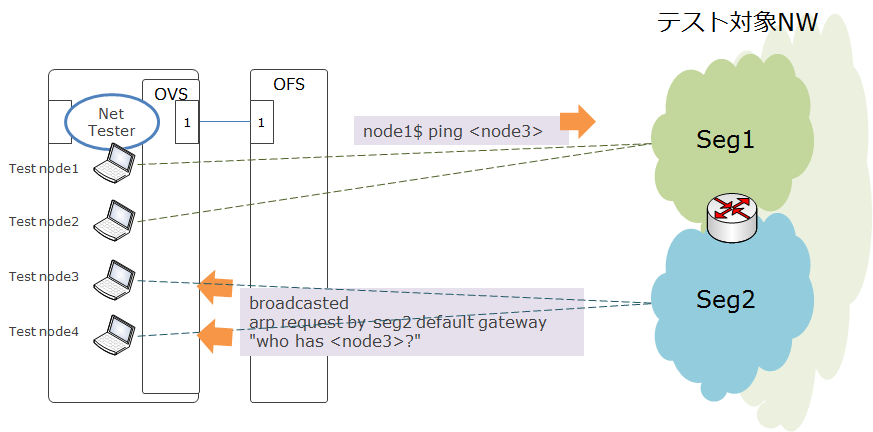
\includegraphics[scale=0.6]{img/l2bcctrl_req1.png}
 \caption{L2 Broadcast 制御の要件}
 \label{fig:l2bcctrl_req1}
\end{figure}

テスト用ノードを増やしていったときに、テスト対象ネットワークにある機器側
で接続先物理ポートが都度必要になってしまうと、拡張性を制限する原因となっ
てしまう。テストシステムでは、自由に・多数のテスト用ノードを生成し、かつ、
物理ポートの利用を抑えるようにしたい。そのために、テスト用ノードではVLAN
による複数セグメントの集約を利用できるようにする
(\figref{fig:l2bcctrl_req2})。

\begin{figure}[h]
 \centering
 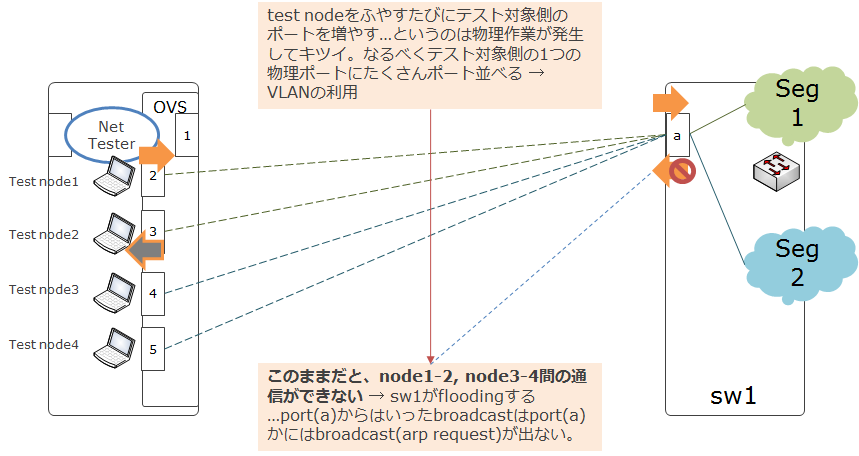
\includegraphics[scale=0.6]{img/l2bcctrl_req2.png}
 \caption{パッチパネル動作上の制約}
 \label{fig:l2bcctrl_req2}
\end{figure}

VLAN の制御については後述するが、
% TODO: ref
\figref{fig:l2bcctrl_req2}のようにした場合、テスト対象機器(DUT)の同一物
理ポートに接続したテスト用ノード(ノード1/2, 3/4)の間では相互に通信ができ
ないという制約が発生する。これは、フラッディング動作による。たとえばノー
ド1が送信したブロードキャストはノード2にはフラッディングされない。したがっ
て、ノード1/2は相互にARPをやりとりすることができない。

この問題を解決するためには、同一機器(DUT)・同一セグメントでの通信をおこ
ないたい場合は\figref{fig:l2bcctrl_req3}のような構成をとる。詳細について
は \lopjtech を参照すること。

\begin{figure}[h]
 \centering
 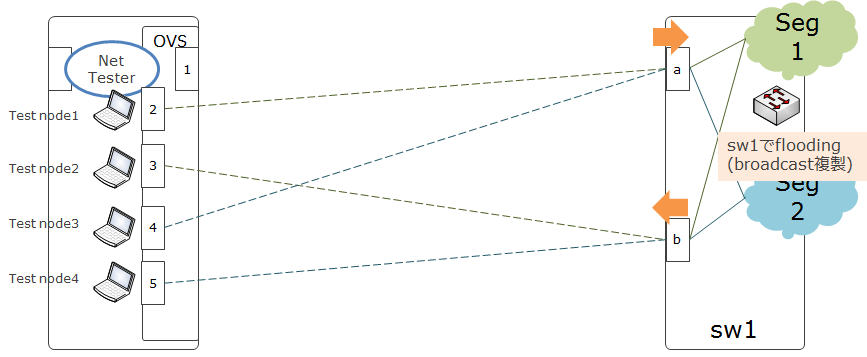
\includegraphics[scale=0.6]{img/l2bcctrl_req3.png}
 \caption{テスト用ノード配置の要求}
 \label{fig:l2bcctrl_req3}
\end{figure}

ブロードキャストは、実際には物理スイッチとソフトウェアスイッチの間の物理
リンクを経由して転送される。4台のテスト用ノードがひとつのセグメントに所
属していて、ノード4のみが異なる物理ポートでパッチ接続されている状況を考
える(\figref{fig:l2bcctrl_req4})。このとき、Seg.1で発信されたブロードキャ
ストは、ポート(a)とポート(b)からそれぞれ出力される。このふたつのブロード
キャスト(フレーム)は物理スイッチからソフトウェアスイッチへ転送され、ノー
ド1-4へ転送されなければならない。

システム構成上、物理スイッチとソフトウェアスイッチの間はひとつの物理リン
クのみとする(\ref{sec:nettester-model-restriction}節参照)。OpenFlowでは、
同一のポートにパケットの複製して複数ながすことはできないため、ソフトウェ
アスイッチで各テストノードむけにパケットを複製して送信する必要がある。

\begin{figure}[h]
 \centering
 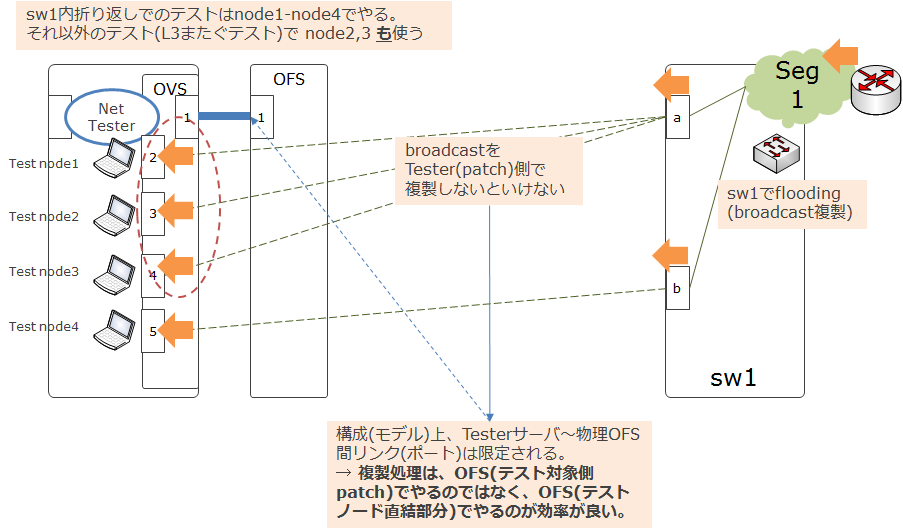
\includegraphics[scale=0.6]{img/l2bcctrl_req4.png}
 \caption{L2 Broadcast パケット複製ポイント}
 \label{fig:l2bcctrl_req4}
\end{figure}

「パッチパネル」では、接続された2点(2ポート)間が1:1に接続される。
\figref{fig:l2bcctrl_req4}ではポート(a)(b)から送信されたSeg.1内のブロー
ドキャストが2フレームソフトウェアスイッチに転送されるが、「パッチパネル」
としてはこれを同じものとして扱うのは望ましくない。パッチ接続の対応関係に
基づいて、ポート(a)から送信されたブロードキャストフレームはノード1-3へ、
ポート(b)から送信されたブロードキャストフレームはノード4へと、それぞれ転
送されるのが「パッチパネル」としての理想的な動作となる。

  \subsection{Broadcast制御 案1/簡易制御}
  \label{sec:l2bcctrl-plan1}

\ref{sec:l2bcctrl-requirement}節に、「パッチパネル」動作に基づいてブロー
ドキャスト制御に制御されるのが理想的かを示した。しかし、この理想的な動作
をやや緩和することで、ブロードキャスト制御の実装が非常にシンプルにできる。

案1/簡易制御では、\figref{fig:l2bcctrl_req4}と同様の状況で、ポート(a)(b)
から送信されるブロードキャストフレーム(a)(b)を区別しない。これらはいずれ
も Seg.1 内にブロードキャストであり、どちらも同様に Seg.1 に属するノード
(ノード1-4)へ複製・転送する(\figref{fig:l2bcctrl_plan1_design})。

\begin{figure}[h]
 \centering
 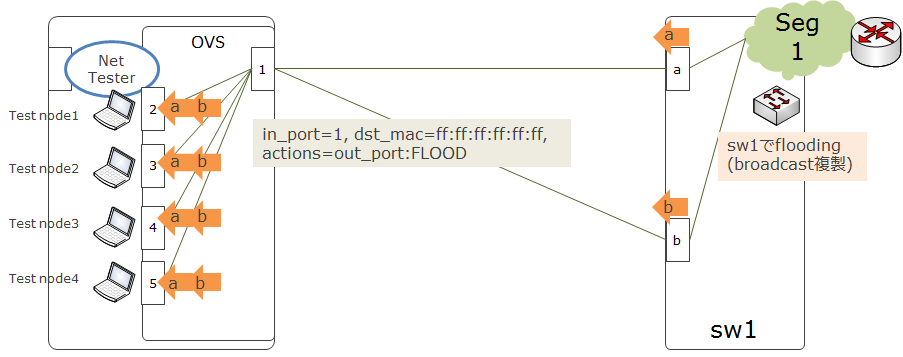
\includegraphics[scale=0.6]{img/l2bcctrl_plan1_design.png}
 \caption{Broadcast制御 案1/簡易制御}
 \label{fig:l2bcctrl_plan1_design}
\end{figure}

そのため、Seg.1(テスト対象NW)内で複製されたブロードキャストフレーム
(a)(b)は都度複製され各テスト用ノードに送信される。この動作は、ソフトウェ
アスイッチ上ではひとつのルールでノード数によらず固定で記述できるため、フ
ロールールの実装上は非常にシンプルになる。

  \subsection{Broadcast制御 案2/Wire-group制御}
  \label{sec:l2bcctrl-plan2}

\ref{sec:l2bcctrl-requirement}節に示したように、ブロードキャストは対応す
るセグメントおよびパッチ接続先(DUT物理ポート)に応じて複製・転送されるの
が望ましい。\lopjc ではこの理想的な動作を実現するために、wire-group とい
う情報を付与して、パッチ接続単位のブロードキャスト制御を実装した
(\figref{fig:l2bcctrl_plan2_design})。

\begin{figure}[h]
 \centering
 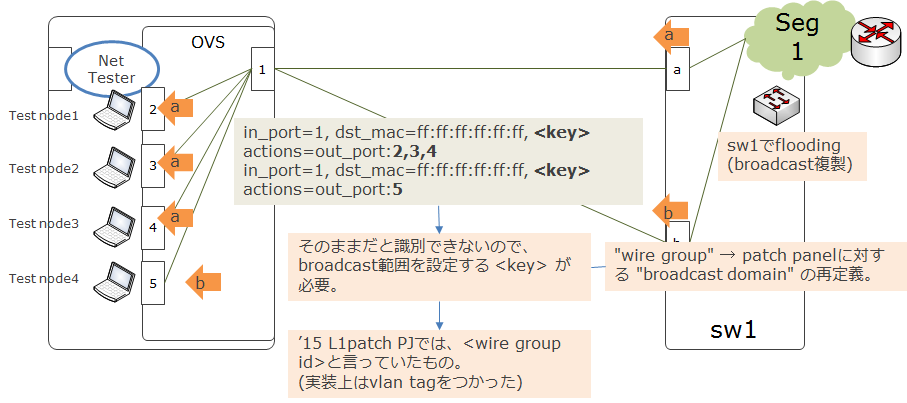
\includegraphics[scale=0.6]{img/l2bcctrl_plan2_design.png}
 \caption{Broadcast制御 案2/Wire-group制御}
 \label{fig:l2bcctrl_plan2_design}
\end{figure}

Wire-group には VLAN Tag を使用している。テスト対象ネットワーク内でつか
うVLAN Tagとは異なる使いかたなので、タグのつけはずしなどの処理をおこなう
(詳細は \lopjtech を参照すること)。したがって、テスト用ノードの設定・パッ
チ設定に応じてフロールールが変動し、案1にくらべてフロー制御は複雑になる
(\figref{fig:l2bcctrl_plan2_implement})。

\begin{figure}[h]
 \centering
 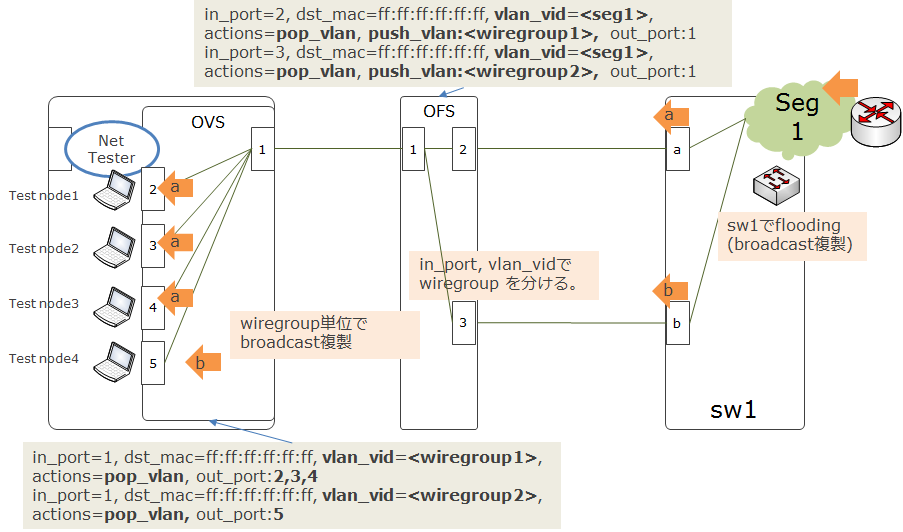
\includegraphics[scale=0.6]{img/l2bcctrl_plan2_implement.png}
 \caption{Broadcast制御 案2/Wire-group制御(実装)}
 \label{fig:l2bcctrl_plan2_implement}
\end{figure}

  \subsection{Broadcast制御案の比較と選択}
  \label{sec:l2bcctrl-compare}

案1(\ref{sec:l2bcctrl-plan1}節)・案2(\ref{sec:l2bcctrl-plan2}節)のメリッ
ト・デメリットをまとめてみると\tabref{tab:l2bcctrl_compare}のようになる。
本プロジェクトでは、その目的(\ref{sec:behavior-test}節)からツールとして
の機能・拡張性よりもユースケース実証に重きをおく。そのため、構成のシンプ
ルさにみあった制御ルールのシンプルさが得られる案1を採用した。

\begin{table}[h]
 \caption{L2 Broadcast 制御案 比較}
 \label{tab:l2bcctrl_compare}
 \centering
 \begin{tabularx}{\linewidth}{c|X|X}
  \hline
  案 & メリット & デメリット \\ \hline
  \hline
  案1 & 実装がシンプル
      & 「パッチパネル」としての動作としては理想的ではない。ブロードキャストが多数あるとパケット複製処理のオーバーヘッドがおおきく性能面での影響が予想される。 \\ \hline
  案2 & 「パッチパネル」として理想的な動作であり不要なブロードキャストの複製を抑制できる。
      & NetTesterのシステム構成のシンプルさに対して実装が複雑になる。 \\ \hline
 \end{tabularx}
 \end{table}

複数OpenFlowスイッチ・DUTポート単位でのブロードキャスト制御(案2)について
は、\lopj で実証できている。本プロジェクトでユースケースを実証し、より複
雑なシステム構成、拡張性が必要になった際は、案2を使用して制御ロジックを
再実装することで実現が可能である。

  \subsection{フロー制御設計の注意事項}
  % https://drive.google.com/file/d/0B2eRR_JxYJA5TmhaeWItNF93Um8/view
  % 図, 補足: bcast/案1派生のところ。
  % フロールールから: arp があるていどみえてしまうこと → セキュリティについて?

  \paragraph{Broadcast制御の選択肢}

テスト対象ネットワーク(Testee)からテスト用ノード(Tester)へ送信されるブロー
ドキャストの複製についてみてきた。検討点としてはTesterからTesteeへのブロー
ドキャストについて、ソフトウェアスイッチ内で複製させることも可能である
(\figref{fig:bcctrl_another_pattern})。

\begin{figure}[h]
 \centering
 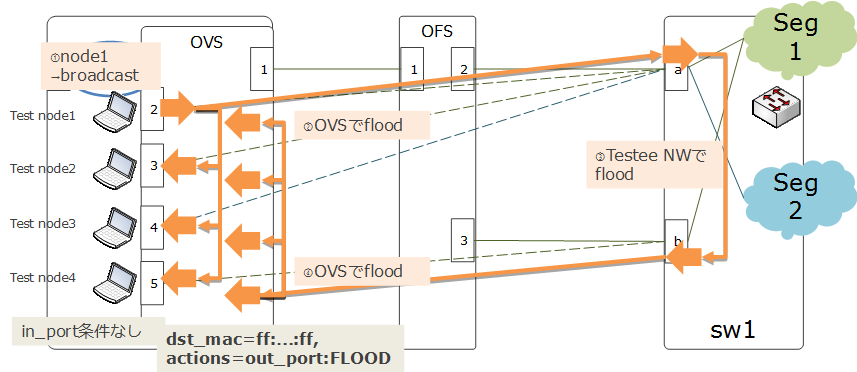
\includegraphics[scale=0.6]{img/l2bcctrl_another_pattern.png}
 \caption{テスト用ノードのブロードキャスト制御パターン}
 \label{fig:bcctrl_another_pattern}
\end{figure}

\figref{fig:bcctrl_another_pattern}ではソフトウェアスイッチ(OVS)では入力
ポート(\code{in\_port})条件を指定せず、ブロードキャストを常にフラッディ
ングする。フロー制御ルールとしてはよりシンプルになるが、今回は以下の理由
からソフトウェアスイッチ内でのブロードキャスト折り返しは採用していない。
\begin{itemize}
 \item ソフトウェアスイッチ内だけでなく、テスト対象ネットワーク内でもブ
       ロードキャストが複製され、テスト用ノードに多数の(不用な)ブロード
       キャストフレームがコピーされる。
 \item 「パッチパネル」をモデルとしたトラフィック制御をしているため、理
       想としては、ある「パッチ」でやりとりされているデータは異なる「パッ
       チ」で接続されるノードには見えてはいけない。
 \item テスト対象ネットワーク内でブロードキャストが正しくおこなわれ、テ
       スト用ノードに送信されるかどうかも、テストとして確認したいことに
       含まれる。本来テスト対象ネットワークでおこなわれるべき処理を、テ
       ストシステム(ソフトウェアスイッチ)側で代行してしまうのは、「ネッ
       トワークのテスト」という目的からは避けなければいけない。
       \footnote{ソフトウェアスイッチでテスト用ノード間のブロードキャス
       ト折り返しを許可してしまうと、テスト対象ネットワーク側の不具合な
       どでL2の接続ができない状態になっていても、あるテスト用ノードから
       隣にいるテスト用ノードのMACが見えるという状況が発生し得る。これは
       従来の、独立した機器をテスト対象に直接結線していた状況では発生し
       ない。テストシステムとしては、「本来パッチパネルで直接接続されて
       いたときに想定されること」を再現することが望ましい。}
 \item ソフトウェアスイッチと物理スイッチの間のリンクについて、NetTester
       では1本と設定しているが、複数本に拡張するとL2ループとなる。構成次
       第ではあるが、無条件のフラッディングはブロードキャストストームに
       発展しやすいというリスクがある。
\end{itemize}

\paragraph{設計上の注意事項}

テストシステムとしては「パッチパネル」でテスト対象にテスト用ノードを直接
接続した状況を忠実に再現できることが理想である。しかし、今回選択したフロー
制御ルール(\ref{sec:l2bcctrl-plan1}節; 案1)では、テスト対象ネットワーク
からテスト用ノードへのブロードキャストについては本来の「パッチパネル」の
動作からははずれた動作をする。具体的には、あるテスト用ノードが接続されて
いる「パッチ」には流れないはずのブロードキャストも、ソフトウェアスイッチ
で複製されてしまう。そのため、本来見えないはずの隣接ノードの情報(MACアド
レス)なども見えてしまう。

本プロジェクトでは、PoC(ユースケースの実証)を主要な目的とし、実装上は可
能な限りシンプルにすることを方針としたため、こうした動作については許容す
ることとした。また、\lopj ではwire-groupによるブロードキャスト範囲の制限
を試みており、より詳細なコントロールも可能であることも理由として挙げられ
る。
% TODO, ref:PoC


 \section{トラフィック転送とVLANの制御設計}
 \label{sec:vlan-ctrl}

\ref{sec:l2bcctrl-requirement}節に示したように、構成上の物理リソース(物
理ポート/リンク)消費を抑えるために、テスト対象ネットワーク側でVLANを利用
し、ひとつの物理ポートで複数のセグメントを集約する。このときのユニキャス
トの制御およびブロードキャストの制御(案1: \ref{sec:l2bcctrl-plan1}参照)
を検討する。

  \subsection{VLAN利用の要件}
  \label{sec:vlan-ctrl-req}

例として、4台のテスト用ノードがテスト対象ネットワークの2つのセグメントに
パッチ接続されている状況を想定する(\figref{fig:vlan-req})。このとき、ポー
ト(a)は vlan tagged port (trunk port)、ポート(b)は untagged port (access
port) である。ノード1-2はSeg.1、ノード3はSeg.2に所属している。また、
sw1/Seg.1内の折り返し通信をおこなうため、ノード4をポート(b)に配置する。

\begin{figure}[h]
 \centering
 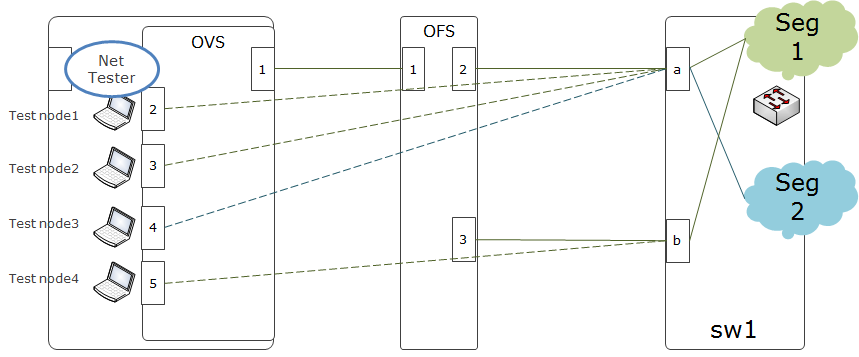
\includegraphics[scale=0.6]{img/vlan-req.png}
 \caption{VLAN制御の要件}
 \label{fig:vlan-req}
\end{figure}

VLAN Tagをどこでテスト用ノードで制御することも可能だが、\lopjc では以下
の理由からOpenFlow スイッチ(物理スイッチおよびソフトウェアスイッチ)で
VLAN Tagの制御をおこなっていた。NetTesterの実装もこれに従っている。
\begin{itemize}
 \item テスト用ノードとしてVLAN Tagを利用できないノードも想定する。
 \item Wire-group(\ref{sec:l2bcctrl-plan2}節)をつかった制御では、
       wire-group の情報をVLAN Tag を使用して実装する。そのため、VLAN
       Tagの制御を物理スイッチ・ソフトウェアスイッチの両方でおこなう必要
       がある。
\end{itemize}

  \subsection{TesterからTesteeへ向かうトラフィックのVLAN制御}
  \label{sec:vlan-ctrl-tester2testee}

Tester(テスト用ノード)が送信したトラフィックをTestee(テスト対象ネットワー
ク)に送信する場合、ユニキャスト/ブロードキャストともに送信元の情報
(Source MAC)が一意に定まる。パッチとしての接続先(物理スイッチのポート番
号)は与えられるため、これをもとに転送制御できる
(\figref{fig:vlan-tester2testee})。

ポート(a)に接続するパッチについて、VLAN Tagは物理スイッチ/ソフトウェアス
イッチどちらで設定してもよい。

\begin{figure}[h]
 \centering
 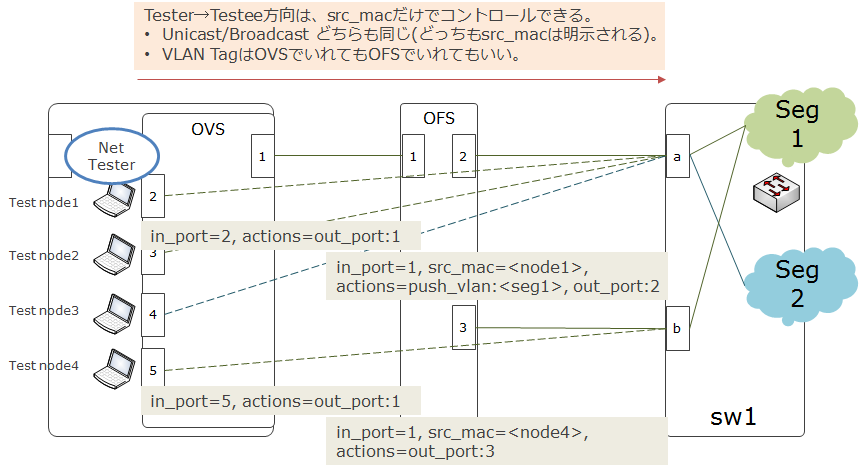
\includegraphics[scale=0.6]{img/vlan-tester2testee.png}
 \caption{Testeeへ向かうユニキャスト/ブロードキャストのVLAN制御}
 \label{fig:vlan-tester2testee}
\end{figure}

  \subsection{TesteeからTesterへ向かうユニキャストのVLAN制御}
  \label{sec:vlan-ctrl-testee2tester-unicast}

TesteeからTester(テスト用ノード)ヘ向かうトラフィックは、ユニキャストとブ
ロードキャストで制御が異なるため分けて扱う。Tester宛てのユニキャストは、
送信先(Destination MAC)が一意に識別できるため、これをもとに転送制御でき
る(\figref{fig:vlan-testee2tester})。

ポート(a)に接続するパッチについて、VLAN Tagは物理スイッチ/ソフトウェアス
イッチどちらで設定してもよい。

\begin{figure}[h]
 \centering
 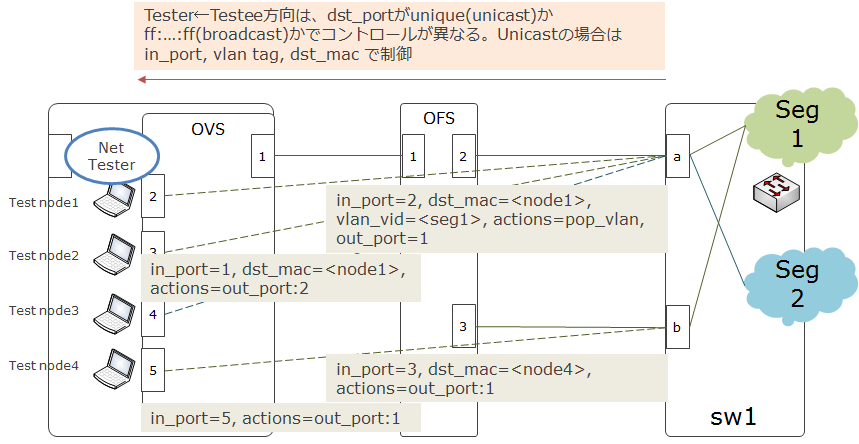
\includegraphics[scale=0.6]{img/vlan-testee2tester.png}
 \caption{Testerへ向かうユニキャストのVLAN制御}
 \label{fig:vlan-testee2tester}
\end{figure}

  \subsection{TesteeからTesterへ向かうブロードキャストのVLAN制御}
  \label{sec:vlan-ctrl-testee2tester-broadcast}

Tester(テスト用ノード)に向かうブロードキャストは、宛先(Destination MAC)
がブロードキャストアドレスとなるため、一意には定まらない。パッチ(送信元
情報: どこのTestee portから送信されるか)とセグメント(VLAN ID)をもとにブ
ロードキャストの複製・転送先を判断する必要がある
(\figref{fig:vlan-testee2tester-bcplan1})。

ブロードキャスト制御として案1(\ref{sec:l2bcctrl-plan1}節)を採用するため、
ソフトウェアスイッチに設定するブロードキャスト制御のルールは、原則
\verb|in_port=1, actions=FLOOD|のルールのみとなる。
\begin{figure}[h]
 \centering
 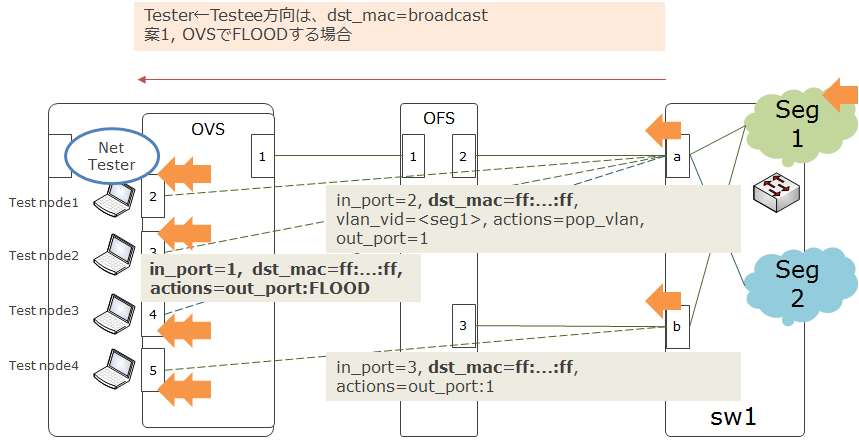
\includegraphics[scale=0.6]{img/vlan-testee2tester-bcplan1.png}
 \caption{Testerへ向かうブロードキャストのVLAN制御}
 \label{fig:vlan-testee2tester-bcplan1}
\end{figure}

\figref{fig:vlan-testee2tester-bcplan1}では物理スイッチ側でTesteeから送
信されたフレームのVLAN Tagをはずす処理をしているが、どこでVLAN Tagのつけ
はずしをおこなうかによって実装が変化する(VLAN制御ポイントや実装比較につ
いては\ref{sec:vlan_control_point}節)。いずれにせよソフトウェアスイッチ
で\verb|actions=FLOOD|とするため、ブロードキャストはセグメントによらず全
てのテスト用ノードへ送信される。

  \subsection{VLAN制御ポイントの比較}
  \label{sec:vlan_control_point}
  % NetTester-build-simple-broadcast-control
  % https://docs.google.com/spreadsheets/d/1cipE5Q_1N5vpRaepBgQR2s03dcJBeBpG-XUsHTEzf8A/edit#gid=1208238463

\ref{sec:vlan-ctrl-req}節-\ref{sec:vlan-ctrl-testee2tester-broadcast}節
で示したように、ブロードキャスト制御案1(\ref{sec:l2bcctrl-plan1}参照)の
元では、VLAN tagの制御は物理スイッチ/ソフトウェアスイッチのどちらでも実
装が可能である。
\tabref{tab:vlan-ctrl-by-ssw}にソフトウェアスイッチ(SSW)でVLAN Tag操作す
る場合のフロールールを、\tabref{tab:vlan-ctrl-by-psw}に物理スイッチ(PSW)
でVLAN Tag操作する場合のフロールールを示す。NetTester では、以下の理由か
ら SSW による VLAN Tag 操作を採用している。
\begin{itemize}
 \item 物理スイッチはスイッチOSやハードウェア(ネットワークチップ)などに
       より、製品ごとに機能差があることがある。今回はOpenFlowでも最も基
       本的なOpenFlow/1.0およびVLAN Tag操作程度の機能しか使っていないた
       め、リスクは少ないと考えられるが、複雑な処理が確実に動作するソフ
       トウェア処理のSSW側に寄せる。
 \item SSW側でVLAN Tag操作をおこなうほうが、システム全体のフロールールを
       シンプルにできる(フローの設定項目を少なくできる)。
\end{itemize}

\begin{landscape}
 \begin{table}[h]
  \centering
  \caption{SSWでVLAN Tag操作をおこなう場合}
  \label{tab:vlan-ctrl-by-ssw}
  \begin{threeparttable}
   \begin{tabularx}{\linewidth}{p{5em}|p{5em}|c|X|X}
    \hline
    Direction & Type & VLAN & Flow rule @SSW & Flow rule @PSW \\
    \hline
    \hline
    Tester to Testee & Unicast \& Broadcast & None
      & (1) \code{in\_port=\#p, actions=out\_port:1}
      & (2) \code{in\_port=1, src\_mac=\#host\_mac, actions=out\_port:\#q} \\
    \cline{3-5}
    & & Exist
      & (3) \code{in\_port=\#p, actions=SetVlanVid:\#v,out\_port:1}
      & \cellcolor{gray}
        (4) \code{in\_port=1, src\_mac=\#host\_mac, vlan\_vid=\#v, actions=out\_port:\#q}, (2)に含まれる。 \\
    \hline
    Testee to Tester & Unicast & None
      & (5) \code{in\_port=1, dst\_mac=\#host\_mac, actions=out\_port:\#p}
      & (6) \code{in\_port=\#q, actions=out\_port:1} \\
    \cline{3-5}
    & & Exist
      & (7) \code{in\_port=1, dst\_mac=\#host\_mac, vlan\_vid=\#v, actions=StripVlanHeader,out\_port:\#p}
      & \cellcolor{gray}
        (8) \code{in\_port=\#q, dst\_mac=\#host\_mac, vlan\_vid=\#v, actions=out\_port:1}, (6)に含まれる \\
    \cline{2-5}
    & Broadcast & None
      & (9) \code{in\_port=1, dst\_mac=[broadcast], actions=out\_port:FLOOD}, per-switch rule
      & \cellcolor{gray}
        (10) \code{in\_port=\#q, dst\_mac=[broadcast], actions=out\_port:1}, (6)に含まれる \\
    \cline{3-5}
    & & Exist
      & (11) \code{in\_port=1, dst\_mac=[broadcast], vlan\_vid=\#v, actions=StripVlanHeader, out\_port:FLOOD}, per-wire rule, non-tag broadcast rule (9) より優先にならないと tag strip されずにフラッディングされる。
      & \cellcolor{gray}
        (12) \code{in\_port=\#q, dst\_mac=[broadcast], vlan\_vid=\#v, actions=out\_port:1}, (6)に含まれる \\
    \hline
   \end{tabularx}
   \begin{tablenotes}
    \footnotesize
    \item \verb|#p, #q|: ポート番号
    \item \verb|#v|: VLAN ID
    \item \verb|#host_mac|: テスト用ノードのMACアドレス
    \item \verb|[broadcast]|: Broadcast MAC Address (\verb|ff:ff:ff:ff:ff:ff|)
   \end{tablenotes}
  \end{threeparttable}
 \end{table}
\end{landscape}

\begin{landscape}
 \begin{table}[h]
  \centering
  \caption{PSWでVLAN Tag操作をおこなう場合}
  \label{tab:vlan-ctrl-by-psw}
  \begin{threeparttable}
   \begin{tabularx}{\linewidth}{p{5em}|p{5em}|c|X|X}
    \hline
    Direction & Type & VLAN & Flow rule @SSW & Flow rule @PSW \\
    \hline
    \hline
    Tester to Testee & Unicast \& Broadcast & None
      & (1) \code{in\_port=\#p, actions=out\_port:1}
      & (2) \code{in\_port=1, src\_mac=\#host\_mac, actions=out\_port:\#q} \\
    \cline{3-5}
    & & Exist
      & (3) \cellcolor{gray}
            \code{in\_port=\#p, actions=out\_port:1}, (1)同様。
      & (4) \code{in\_port=1, src\_mac=\#host\_mac, actions=SetVlanVid:\#v, out\_port:\#q} \\
    \hline
    Testee to Tester & Unicast & None
      & (5) \code{in\_port=1, dst\_mac=\#host\_mac, actions=out\_port:\#p}
      & (6) \code{in\_port=\#q, actions=out\_port:1} \\
    \cline{3-5}
    & & Exist
      & \cellcolor{gray}
        (7) \code{in\_port=1, dst\_mac=\#host\_mac, vlan\_vid=\#v, actions=out\_port:\#p}, (5)に含まれる。
      & (8) \code{in\_port=\#q, dst\_mac=\#host\_mac, vlan\_vid=\#v, actions=StripVlanHeader,out\_port:1} \\
    \cline{2-5}
    & Broadcast & None
      & (9) \code{in\_port=1, dst\_mac=[broadcast], actions=out\_port:FLOOD}, per-switch rule
      & (10) \code{in\_port=\#q, dst\_mac=[broadcast], actions=StripVlanHeader, out\_port:1}, per-wire rule \\
   \cline{3-5}
   & & Exist
      & \cellcolor{gray}
        (11) \code{in\_port=1, dst\_mac=[broadcast], actions=out\_port:FLOOD}, (9)同様。
      & (12) \code{in\_port=\#q, dst\_mac=[broadcast], vlan\_vid=\#v, actions=StripVlanHeader,out\_port:1}, per-wire rule, non-tag broadcast rule (10) より優先にならないと tag strip されずにフラッディングされる。 \\
    \hline
   \end{tabularx}
   \begin{tablenotes}
    \footnotesize
    \item \verb|#p, #q|: ポート番号
    \item \verb|#v|: VLAN ID
    \item \verb|#host_mac|: テスト用ノードのMACアドレス
    \item \verb|[broadcast]|: Broadcast MAC Address (\verb|ff:ff:ff:ff:ff:ff|)
   \end{tablenotes}
  \end{threeparttable} 
 \end{table}
\end{landscape}


 \section{フロー優先度設計}
 \label{sec:flow-priority-design}
 % Table & Rule Priority Design (2015 ool-l1patch) – NetTester
 % https://3.basecamp.com/3088280/buckets/867009/documents/211290387
 % Table & Rule Priority Design (NetTester) – NetTester
 % https://3.basecamp.com/3088280/buckets/867009/documents/217426690

NetTesterはOpenFlow/1.0を使用するため、ひとつのフローテーブル内で優先度
によるマッチ条件の使いわけをおこなう(\ref{sec:flow-design-premise}節)。
一般的には、マッチ項目が多いルール(より複雑なマッチ条件を持つルール)を優
先させる必要がある。

NetTesterのフロー制御ルールは\tabref{tab:vlan-ctrl-by-ssw}を採用するが、
VLAN Tagがある場合・ない場合でブロードキャストのルールを使いわけ、Tagを
はずすアクションを優先して実行する必要がある。そのため、
\tabref{tab:vlan-ctrl-by-ssw}(11)はVLAN Tagをもたないブロードキャスト制
御ルールとの優先度をわける。OpenFlowではマッチルールにワイルドカードのよ
うな機能がないため、使用するVLAN IDそれぞれについてマッチさせる必要があ
る。

\begin{table}[h]
 \caption{フロールール優先度設計}
 \label{tab:flow-priority-design}
 \centering
 \begin{threeparttable}
  \begin{tabularx}{\linewidth}{c|X|X|X}
   \hline
   優先度 & フロールール種別
      & Flow rule @SSW \tnote{1} & Flow Rule @PSW \tnote{1} \\
   \hline
   \hline
   高 & Tagged broadcast/unicast & (3),(7),(11) & (6) \\ \hline
   中 & Untagged broadcast/unicast & (1),(5),(9) & (2) \\ \hline
   低 & Layer1 \tnote{2} & & \\ \hline
   0(最小) & default(match-any)
      & \multicolumn{2}{c}{\code{actions=DROP} or \code{actions=CONTROLLER}}\\
   \hline
  \end{tabularx}
  \begin{tablenotes}
   \footnotesize
   \item[1] \tabref{tab:vlan-ctrl-by-ssw} No.
   \item[2] 「専有モードワイヤ」(\ref{sec:flow-design-grouping})
  \end{tablenotes}
 \end{threeparttable}
\end{table}

OpenFlow/1.0では、テーブルミス\footnote{フローテーブル内のどのフロールー
ルにもマッチしない場合。}のとき、デフォルトでコントローラに送信
\footnote{\code{actions=CONTROLLER} = OFCへのPacket-in送信}される。この
動作はこのあとの OpenFlow バージョンでは変更されているので、NetTester
OFCでは動作を統一させるために明示的に指定する。当初、デバッグ用途もあり
\code{actions=CONTROLLER}としていたが、Trema のパケットパーサ(Trema/Pio)
で特定のパケットがパースできず、コントローラが停止するバグがあった
\footnote{修正済。デバッグについての補足情報については
\ref{sec:debugging-trema}節を参照。}ため、NetTesterでは default DROP を
採用している。

  \section{リンク操作方式}
  \label{sec:link-operation}

  % テスト対象NW機器間接続のup/down方式を決める – NetTester
  % \url{https://3.basecamp.com/3088280/buckets/867009/todos/238171702}
  % リンクダウン・リンクアップ機能用のスクリプト実装 – NetTester
  % \url{https://3.basecamp.com/3088280/buckets/867009/todos/247379766}

  % https://drive.google.com/file/d/0B2eRR_JxYJA5TmhaeWItNF93Um8/view
  % 図、NW機器間接続

\tabref{fig:features-of-network-testing} No.3では物理リンク(物理トポロジ)操
作をあげた。これは、複数のポートをつなぎあわせて(「パッチ」して)テスト対
象ネットワークの物理トポロジを構成するという観点だけでなく、テスト中に発
生する物理リンク操作という観点も含まれる(\ref{sec:behavior-to-test}節
「動的なふるまい」参照)。ここでは「動的なふるまい」のテストのための物理
リンク操作方法について解説する。

テスト対象ネットワークでは\figref{fig:patch-layer1}のように、物理
OpenFlowスイッチを仲介させることで物理トポロジ操作を可能にする。このとき、
「動的なふるまい」を発生させるために、NW機器間のリンクを操作する。あたら
しくリンクを追加する場合は同様に物理OpenFlowスイッチへの結線とフロールー
ルの追加をおこなう。リンクを削除する場合には以下の2パターンが考えられる。
\begin{description}
 \item[直接リンクダウン] 物理OpenFlowスイッチのポート自体をup/downさせる
            ことでリンクを操作する。この場合、テスト対象ネットワーク機器
            側でもポートのup/downを直接検出することができる。
 \item[関節リンクダウン] 物理OpenFlowスイッチで、リンクを成立させている
            ポート間マッピングのためのフロールールをadd/deleteする。この
            場合、テスト対象ネットワーク機器側ではリンクの状態変更
            (up/down)は発生せず、トラフィックが送受信できない状態となる。
\end{description}

\begin{figure}[h]
 \centering
 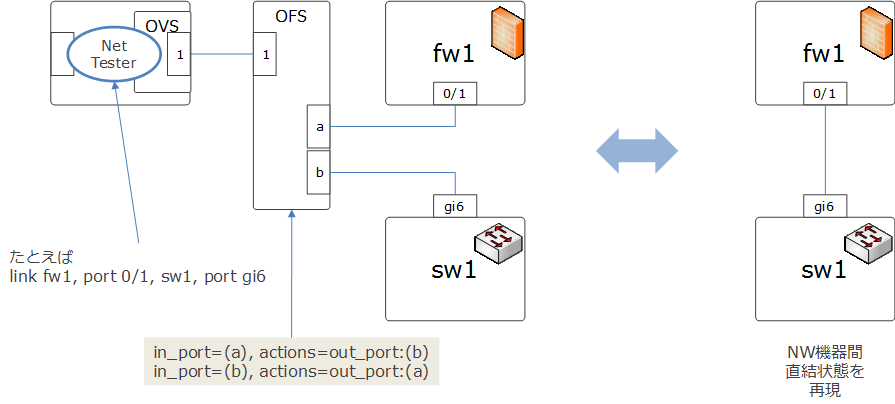
\includegraphics[scale=0.6]{img/patch-layer1.png}
 \caption{テスト対象の物理トポロジ操作}
 \label{fig:patch-layer1}
\end{figure}

本プロジェクトでは、PoCとして、最も基礎となる「動的なふるまい」とそのテ
ストをターゲットとし、リンク障害試験をそのユースケースとしてとりあげた。
リンク障害は通常、テスト対象ネットワーク内(該当するリンクをもつネットワー
ク機器)でポートのup/downを検出するため、直接リンクダウン方式を採用する。

直接リンクダウンの実装としては、以下の2つの方法がある。
\begin{itemize}
 \item 物理OpenFlowスイッチ上でポート状態操作コマンドを実行する。
 \item OpenFlow Message (PortMod) を物理OpenFlowスイッチに送信し、ポート
       状態変更操作をおこなう。
\end{itemize}
今回、NetTester では、物理OpenFlowスイッチにExpectベースのツール
(\ref{sec:expectacle}節)でログイン/コマンド実行し、直接スイッチ上でポー
ト状態変更する方法をとった。これは、PoC実施時点\footnote{2016年10月-12月}の
TremaではまだPortModメッセージの送信が実装されていなかったためである。

%% TODO/あと、以下のはなしどうする?

% NetTester 自体の通信要件?
% \begin{itemize}
%  \item openflow, ssh, syslog 等
% \end{itemize}

% 複数プロセス同時実行とかの技術使用ベースの話とかはどこで書く?

%%% Local Variables:
%%% mode: yatex
%%% TeX-master: "main.tex"
%%% End:
